\documentclass[mathserif,handout]{beamer}
%\documentclass{beamer}
\usetheme{Warsaw}
\usecolortheme{seahorse}
\usecolortheme{orchid}
\usepackage{amsmath,verbatim}
\usepackage{listings}
\usepackage[english]{babel}
\usepackage{movie15}
\setbeamercovered{transparent}

\newcommand{\Deltap}{\ensuremath{\Delta^{\!+}}}
\newcommand{\trans}{\ensuremath{{}^\mathrm{T}}}
\newcommand{\eps}{\varepsilon}
\newcommand*{\approxdist}{\mathrel{\vcenter{\offinterlineskip
\vskip-.25ex\hbox{\hskip.55ex$\cdot$}\vskip-.25ex\hbox{$\sim$}
\vskip-.5ex\hbox{\hskip.55ex$\cdot$}}}}

\lstdefinelanguage{myR}
{
   language=R,
   otherkeywords={read.table, set.seed, head},
   deletekeywords={url,codes, t, dt, Call, formula,Q, R, on,by,hat,is,
col, set,start,end,deltat,zip},
   sensitive=true,
   breaklines=true,
   morecomment=[l]{\#},
   morestring=[b]",
   morestring=[b]',
   basicstyle =\ttfamily\small,
   keywordstyle=\bfseries,
   showtabs=false,
   showstringspaces=false,
   literate= {~}{$\sim$}{2},
   numberstyle=\sffamily\scriptsize,
   stepnumber=2
 }

\lstset{basicstyle=\ttfamily\color{blue}}

\begin{document}

\title[Reactive streams and POMP models]{Reactive streams and POMP models as fundamental building blocks of IoT systems}
\author[Darren Wilkinson --- IoT Systems, 13/1/16]{\textbf{\large Darren Wilkinson} \\
\url{@darrenjw}\\
\alert{\url{http://tinyurl.com/darrenjw}}\\
School of Mathematics \& Statistics\\Newcastle University, UK}
\date{IoT Systems Workshop\\Doxford Hall, Northumberland\\ 11th--13th January 2016}

\frame{\titlepage}

\section{Introduction}

\subsection{Outline}

\frame{
\frametitle{Talk outline}
\begin{itemize}
\item Internet of Data
\item How statisticians think about (time series) data
\item State space models and signal processing
\item Continuous time modelling and POMPs
\item On-line versus off-line algorithms
\item Streaming data and flow graphs
\item Lambda architectures
\end{itemize}
}

\subsection{Internet of Data}

\frame{
\frametitle{It's all about the data!}
\begin{itemize}
\item Why bother developing the Internet of Things (IoT) and Internet of Everything (IoE)?
\item Why connect things to the Internet?
\item Connecting to the Internet allows \alert{communication of data}:
  \begin{itemize}
  \item From device to device
  \item From device to/from server
  \item From servers to/from people
  \end{itemize}
\item For devices which communicate directly with people without the need for any additional data or information, then you really don't need the Internet
\item So IoT/IoE are really about communication of data to/from devices --- really the \alert{Internet of Data}
\end{itemize}
}

\section{State space modelling}

\subsection{Time series and state space modelling}

\frame{
\frametitle{Time series and state space modelling}
\begin{itemize}
\item For most IoT applications, \alert{time} is an important attribute of the data being communicated
\item Being able to store, process, query and communicate data in \alert{time order} is vital
\item Many methods from \alert{time series} analysis, \alert{state space modelling} and \alert{signal processing} allow inference for underlying signals, \alert{stochastic states} and \alert{parameters} of inferential interest from \alert{noisy} measurements and data in time
\item State space models acknowledge that the (raw) data and measurements from sensors are typically \alert{not} themselves the quantities of \alert{direct} inferential interest
\item Most established methods assume that data is present on a \alert{regular time grid} --- extension to \alert{irregular observations} is sometimes non-trivial but usually possible
\end{itemize}
}

\frame{
\frametitle{State space models}
\begin{itemize}
\item In classical state space models (SSMs) you have:
  \begin{itemize}
  \item Time course \alert{data}: $y_1, y_2, y_3, \ldots, y_T$
  \item (Unknown) underlying world \alert{state}, $x_t, t=1,2,\ldots,T$
  \item Fixed (but possibly unknown) model \alert{parameters} $\theta$ (all potentially vectors)
  \item A stochastic process \alert{model} $f(x_t|x_{t-1},\theta)$ governing the time-evolution of world state
  \item An \alert{observation model} $g(y_t|x_t,\theta)$ describing the \alert{likelihood} of observations \alert{conditional} on the state (and model parameters)
  \end{itemize}
\item This is a \alert{generative model} in the sense that it can be used to stochastically \alert{simulate} synthetic world state trajectories and data
\item Generative models can be \alert{inverted} using \alert{Bayesian statistics} in order to make inferences for the (current) world state (and possibly fixed parameters) given (all of) the observed data
\end{itemize}
}

\frame{
\frametitle{Simplest possible example...}
\begin{itemize}
\item \alert{Steady state model}:
  \begin{itemize}
  \item State evolution: $x_t = x_{t-1} + \nu_t$
  \item Observation equation: $y_t = x_t + \eps_t$
  \item Generative in the sense that we can simulate next world state and next observation sequentially to produce a \alert{synthetic dataset} consistent with the model
  \end{itemize}
\item Can be inverted using Bayesian reasoning to get an update equation often known as \alert{exponential smoothing}:
  \begin{itemize}
  \item $\hat{x}_t = \alpha y_t + (1-\alpha)\hat{x}_{t-1} $
  \item Function of \alert{all} previous observations, but the influence of any particular observation decays away exponentially as you look back further into the past
  \item $\alpha$ is (a function of) the fixed model parameter and determines the weight of each data point (depends on signal-to-noise ratio)
  \item Learning about the state can be done simply and sequentially as each data point arrives, but learning $\alpha$ usually done off-line
  \end{itemize}
\end{itemize}
}

\frame{
\frametitle{Model ingredients}
\begin{itemize}
\item State evolution modelling:
  \begin{itemize}
  \item Evolving stochastic dynamics with slowly evolving trends
  \item Seasonal components (eg. daily and/or weekly and/or yearly cycles)
  \item Non-linear dynamics
  \item Abrupt jumps and discontinuities
  \end{itemize}
\item Observation models:
  \begin{itemize}
  \item \alert{Noisy} (Gaussian) observations
  \item Poisson models for \alert{count} data
  \item Bernoulli models for \alert{binary} observations (leading to dynamic logistic regression)
  \end{itemize}
\item Models are \alert{composable}
\end{itemize}
}

\subsection{POMP models}

\frame{
\frametitle{POMP models}
\begin{itemize}
\item Classical SSMs assume that the data are on an regular equispaced time grid, so that the state evolution model $f(x_t|x_{t-1},\theta)$ represents a single \alert{time step} of the process
\item Many sensors and devices do not generate data on a regular grid, either by design, or due to crashes/reboots creating large \alert{gaps} of missing values, pushing observations onto a \alert{misaligned grid}, or changes in \alert{sampling frequency}, etc.
\item \alert{Partially observed Markov process} (POMP) models generalise classical SSMs in two important ways:
  \begin{itemize}
  \item The state evolution model formulated in \alert{continuous time}, and is described by a \alert{transition kernel} $f(x_{t+t'}|x_t,t',\theta)$
  \item It is not required that the transition kernel can be \alert{evaluated} --- only that the state process can by stochastically \alert{simulated} forwards in time
  \end{itemize}
\end{itemize}
}

\frame{
\frametitle{Fitting models to data}
\begin{itemize}
\item When it comes to fitting time series models to data, statisticians (and signal processing engineers) make an important distinction between \alert{sequential} (\alert{on-line}) and \alert{batch} (\alert{off-line}) algorithms:
  \begin{itemize}
  \item It is very difficult to learn the fixed model parameters $\theta$ on-line, so this is usually done off-line using algorithms which make many (millions of) passes over (all of) the data
  \item Conditional on $\theta$, it is often possible to solve the dynamic \alert{state estimation} problem sequentially in an on-line manner as each data point becomes available
  \item Even where on-line algorithms are possible, each updating step is typically complex and computationally intensive, and relies on the maintenance of a large state vector
  \end{itemize}
\item On-line algorithms can be used in the context of \alert{streaming data}, but \alert{all} past data is informative for the current state
%\item Neither the on-line nor off-line algorithms use data from small time windows, and neither can be described using simple declarative query languages
\end{itemize}
}

\frame{
\frametitle{Why are SSMs and POMP models useful?}
\begin{itemize}
\item SSMs and POMP models allow \alert{fully probabilistic inference for the world state} using observational data
\item It is the world state that is of key inferential interest, and most questions of \alert{smoothing}, \alert{interpolation}, \alert{imputation}, \alert{prediction}, \alert{forecasting}, \alert{actions}/\alert{alerting} relate to our knowledge of and uncertainty about the world state (now, in the past, and in the future)
\item Actions typically should not be triggered in response to simple functions of the raw data in small time windows, and ``optimal'' decision triggers can not be described using simple declarative query languages operating on the raw data%, and will typically be a function of all of the past data, not just the data in a small recent time window
\item Can quantify \alert{information} in the data, and answer questions relating to the required \alert{sampling frequency} of a constrained sensor/device
\end{itemize}
}

\subsection{Illustrative examples}

\frame{
\frametitle{Comfortable working temperature}
\begin{itemize}
\item An office contains a temperature sensor and an alert is to be triggered when the room temperature becomes uncomfortably hot (over 22 C)
\item Simple trigger: Signal an alert \alert{if there are three readings over 22 in a two minute window}
  \begin{itemize}
  \item Three readings as the sensor is known to be imperfect, but trigger not related to actual temperature in the room, and the rule is vulnerable to a draft of hot air temporarily blowing across the sensor
  \end{itemize}
\item Better trigger: Signal an alert \alert{if the probability that the actual room temperature will exceed 22C in the next 5 minutes is greater than 0.7}
  \begin{itemize}
  %\item Relates to the actual room temperature --- not the sensor readings
  \item SS/POMP model will smooth out short term fluctuations in sensor readings
  \item Historic data on daily/weekly temperature variations together with recent temperature trends allow short term forecasting of future temperature
  \end{itemize}
\end{itemize}
}

\frame{
\frametitle{Server farm scaling}
\begin{itemize}
\item A cluster of nodes in the Cloud is handling a high volume of requests. The cluster load is monitored. When the load gets to high, an additional node should be added to the cluster.
\item Simple trigger: Add a node \alert{if the average measured cluster utilisation over the last 5 minutes exceeded 85\%}
  \begin{itemize}
  \item But you actually want the cluster utilisation to be reasonably high, and you would be quite happy if the cluster load remained at a steady 90\%
  \end{itemize}
\item Better trigger: Add a node \alert{if the cluster utilisation is forecast to exceed 95\% for at least 5 minutes out of the next 30 minutes with a probability of at least 0.7}
  \begin{itemize}
  \item Again, historic patterns can be used to make probabilistic forecasts about future system load in advance of overloading problems
  \end{itemize}
\end{itemize}
}

\section{Architectural implications}

\subsection{Stream processing}

\frame{
\frametitle{Batch processing}
\begin{itemize}
\item For off-line algorithms, such as algorithms for \alert{fixed model parameter inference}, it will be necessary to have the ability to run (arbitrary) complex code over all of the available data
\item Algorithms will typically involve all of the data --- not just data over small time windows
\item It will not typically be possible to describe the algorithms using simple declarative query languages
\item Most algorithms will involve many (millions of) passes over the data, and therefore \alert{in-memory analysis} will be desirable
\item Parameter inference code will need to be re-run periodically
\item Inferred parameters can be used to (re-)calibrate the on-line state estimation and forecasting algorithms
\end{itemize}
}

\frame{
\frametitle{Stream processing}
\centerline{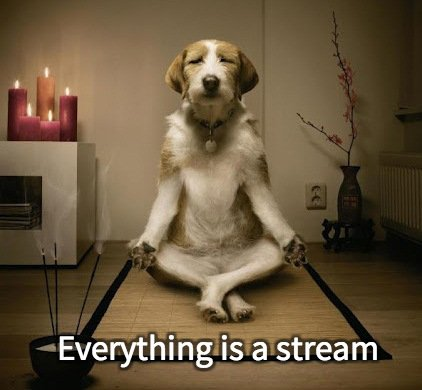
\includegraphics[height=0.8\textheight]{EverythingStream}}
}

\frame{
\frametitle{Stream processing}
\begin{itemize}
\item On-line state estimation algorithms are well-suited to deployment in modern \alert{stream processing frameworks}
\item More generally, stream processing frameworks are a good fit to IoT/IoE data processing
\item \alert{Flow graphs} route data (over the Internet) from \alert{sources} to \alert{sinks} via \alert{flows}
\item On-line signal processing algorithms can be implemented as \alert{flows} to be dropped into the flow graph at an appropriate place --- ideally close to the source if sufficient processing capacity is available, but on a powerful server if necessary
\item Many on-line state estimation algorithms have non-trivial processing requirements in the case of \alert{high-frequency} real-time data processing
\end{itemize}
}

\subsection{Reactive streams}

\frame{
\frametitle{Stream processing}
\begin{itemize}
\item \alert{Functional} programming languages and \alert{design patterns} are well-suited to big data applications, including streaming IoT/IoE data
\item A pure \alert{functional reactive programming} (FRP) approach would be interesting, but it's not (yet) clear how practical that is for robust and resilient production systems
\item The \alert{reactive streams} initiative provides a (cross-platform, language independent) standard for asynchronous stream processing with non-blocking back pressure  (\alert{\url{http://www.reactive-streams.org/}})
\item \alert{Akka Streams} is a good implementation for the JVM --- it has lots of industry support and is the closest thing I know of to FRP that is being used in mainstream production big data systems
\end{itemize}
}

\frame{
\frametitle{Back pressure}
\small
\begin{itemize}
\item Many sensors and other IoT devices are capable of generating data at high-frequency
\item Many on-line statistical algorithms are computationally intensive --- easy to be overwhelmed by a fast incoming data stream
\item Push/pull/push-pull?
  \begin{itemize}
  \item Many stream technologies are \alert{push-based}, but these just block when they overwhelm the consumer
  \item Some stream technologies are \alert{pull-based} (eg. scalaz--stream), but these are slow and inefficient when the consumer can keep pace with the producer
  \item Reactive streams are \alert{push-pull}, behaving like a push-based system when the consumer can keep pace and like a pull-based system when it can't (with demand communicated via a back-channel)
  \end{itemize}
\item Back pressure is useful for stemming the flow when a computationally-intensive on-line algorithm is overwhelmed
%, and also for encouraging a reduced sampling rate from a sensor that is running at an unnecessarily high sampling rate
\end{itemize}
}

\begin{comment}

\frame{
\frametitle{My notes}
\scriptsize
\begin{itemize}
\item IoT really IoD - all about data...
\item Everything is a stream!
\item Time series
\item State space
\item on line versus off line - stream versus batch
\item discrete time versus cts time
\item limitations of "sliding window" methods
\item limitations of querying - non-linear, non-trivial, multiple passes over data, etc.
\item flow graphs
\item statistical models as flows
\item reactive streams
\item sources of back pressure - eg. slow computation or deliberate down sampling
\item FRP
\item lambda architecture
\item Fan-in for joint modelling of multiple series?
\item Limitations of stream based modelling (feedback)
\end{itemize}
}

\end{comment}

% \section{Summary}

\subsection{Summary and conclusions}

\frame{
\frametitle{Summary}
\small
\begin{itemize}
\item Thinking about more sophisticated use cases for IoT systems is helpful for shaping the development of both algorithms and architectures
%\item For algorithm developers:
%  \begin{itemize}
%  \item A lot of IoT data is fundamentally time series data, but methods must be able to cope with data not on a regular time grid
%  \item A greater emphasis needs to be placed on the development of on-line methods for streaming data
%  \end{itemize}
\item For system architects:
  \begin{itemize}
  \item Data measured and recorded typically does not correspond to information of direct inferential interest
  \item Sophisticated algorithms typically do not involve queries on the data over very short time windows and cannot be expressed in simple declarative query languages
  \item Some (but not all) statistical (signal processing) algorithms can operate on-line on streaming data, but are often quite computationally intensive, and may require the maintenance of a significant amount of local state
%  \item Many algorithms need to run off-line on all available data, are very computationally intensive, and may require many (millions of) passes over the data
  \item (Reactive) stream and flow graph processing architectures are useful for on-line methods, and Lambda-like architectures can potentially enable off-line data processing requirements
  \end{itemize}
\end{itemize}
}




\end{document}

